%%%%%%%%%%%%%%%%%%%%%%%%%%%%%%%%%%%%%%%%%%%%%%%%%%%%%%%%%%%%%%%%%%%%%%%%%%%%%%%
%                       CARGA DE LA CLASE DE DOCUMENTO                        %
%                                                                             %
% Las opciones admisibles son:                                                %
%      12pt / 11pt            (tamaño del cuerpo de letra; no usar 10pt)      %
%                                                                             %
% catalan/spanish/english     (idioma principal del trabajo)                  %
%                                                                             % 
% french/italian/german...    (si necesitáis usar otro idioma adicional)      %
%                                                                             %
% listoffigures               (El documento incluye un Índice de figuras)     %
% listoftables                (El documento incluye un Índice de tablas)      %
% listofquadres               (El documento incluye un Índice de cuadros)     %
% listofalgorithms            (El documento incluye un Índice de algoritmos)  %
%                                                                             %
%%%%%%%%%%%%%%%%%%%%%%%%%%%%%%%%%%%%%%%%%%%%%%%%%%%%%%%%%%%%%%%%%%%%%%%%%%%%%%%

\documentclass[11pt,spanish,listoffigures,listoftables]{tfgetsinf}

%%%%%%%%%%%%%%%%%%%%%%%%%%%%%%%%%%%%%%%%%%%%%%%%%%%%%%%%%%%%%%%%%%%%%%%%%%%%%%%
%                     CODIFICACIÓN DEL ARCHIVO FUENTE                         %
%                                                                             %
%    Windows suele usar 'ansinew'                                             %
%    en Linux es posible que sea 'latin1' o 'latin9'                          %
%    Pero lo más recomendable es usar utf8 (unicode 8)                        %
%                                          (si vuestro editor lo permite)     % 
%%%%%%%%%%%%%%%%%%%%%%%%%%%%%%%%%%%%%%%%%%%%%%%%%%%%%%%%%%%%%%%%%%%%%%%%%%%%%%%

\usepackage[utf8]{inputenc} 


%%%%%%%%%%%%%%%%%%%%%%%%%%%%%%%%%%%%%%%%%%%%%%%%%%%%%%%%%%%%%%%%%%%%%%%%%%%%%%%
%                       OTROS PAQUETES Y DEFINICIONES                         %
%                                                                             %
%%%%%%%%%%%%%%%%%%%%%%%%%%%%%%%%%%%%%%%%%%%%%%%%%%%%%%%%%%%%%%%%%%%%%%%%%%%%%%%

\usepackage{glossaries}
\usepackage{textcomp}
\usepackage{booktabs}
\usepackage{float}
\usepackage{enumitem}
\usepackage{graphicx}
\usepackage{subcaption}
\usepackage{tabularx}
\usepackage{pgfplots}
\pgfplotsset{compat=1.18}
\usepgfplotslibrary{groupplots}

\definecolor{localblue}{HTML}{1f77b4}
\definecolor{cloudorange}{HTML}{ff7f0e}

% Bibliografía
\usepackage[backend=biber,style=numeric,sorting=none]{biblatex}
\addbibresource{bibliografia.bib}

% Hyperref siempre al final
\usepackage{hyperref}
\hypersetup{
  colorlinks=true,
  linkcolor=black,
  urlcolor=cyan,
  citecolor=black
}

\usepackage[autostyle=true]{csquotes}
% Listings para código
\usepackage{listings}
\lstset{
  basicstyle=\ttfamily\small,
  frame=single,
  breaklines=true,
  postbreak=\mbox{\textcolor{gray}{$\hookrightarrow$}\space},
  columns=fullflexible,
  keepspaces=true,
  numbers=none,
  literate={á}{{\'a}}1 {é}{{\'e}}1 {í}{{\'i}}1 {ó}{{\'o}}1 {ú}{{\'u}}1
           {Á}{{\'A}}1 {É}{{\'E}}1 {Í}{{\'I}}1 {Ó}{{\'O}}1 {Ú}{{\'U}}1
           {ñ}{{\~n}}1 {Ñ}{{\~N}}1 {¿}{{\textquestiondown}}1 {¡}{{\textexclamdown}}1
}
%%%%%%%%%%%%%%%%%%%%%%%%%%%%%%%%%%%%%%%%%%%%%%%%%%%%%%%%%%%%%%%%%%%%%%%%%%%%%%%
%                          DATOS DEL TRABAJO                                  %
%                                                                             %
% título alumno, titor y curso académico                                      %
%%%%%%%%%%%%%%%%%%%%%%%%%%%%%%%%%%%%%%%%%%%%%%%%%%%%%%%%%%%%%%%%%%%%%%%%%%%%%%%

\title{Comparativa implementación Asistente de Voz: \\Local VS Cloud}
\author{Andrés Pacheco, \\ Miquel Gómez}
% \tutor{No}
% \curs{MUIARFID}

%%%%%%%%%%%%%%%%%%%%%%%%%%%%%%%%%%%%%%%%%%%%%%%%%%%%%%%%%%%%%%%%%%%%%%%%%%%%%%%
%                     PARAULES CLAU/PALABRAS CLAVE/KEY WORDS                  %
%                                                                             %
% Independentment de la llengua del treball, s'hi han d'incloure              %
% les paraules clau i el resum en els tres idiomes                            %
%%%%%%%%%%%%%%%%%%%%%%%%%%%%%%%%%%%%%%%%%%%%%%%%%%%%%%%%%%%%%%%%%%%%%%%%%%%%%%%

\keywords{
    Assistent de veu; LLMs; RAG; Whisper; Kokoro; Ollama; Tavily; AWS; Groq; Hugging Face;
} % Paraules clau 
{
   Asistente de voz; LLMs; RAG; Whisper; Kokoro; Ollama; Tavily; AWS; Groq; Hugging Face;
} % Palabras clave
{
    Voice assistant; LLMs; RAG; Whisper; Kokoro; Ollama; Tavily; AWS; Groq; Hugging Face;
} % Key words


%%%%%%%%%%%%%%%%%%%%%%%%%%%%%%%%%%%%%%%%%%%%%%%%%%%%%%%%%%%%%%%%%%%%%%%%%%%%%%%
%                                                                             %
%                              INICI DEL DOCUMENT                             %
%                                                                             %
%%%%%%%%%%%%%%%%%%%%%%%%%%%%%%%%%%%%%%%%%%%%%%%%%%%%%%%%%%%%%%%%%%%%%%%%%%%%%%%

\begin{document} 


%%%%%%%%%%%%%%%%%%%%%%%%%%%%%%%%%%%%%%%%%%%%%%%%%%%%%%%%%%%%%%%%%%%%%%%%%%%%%%%
%              RESUMENES DEL TFG EN VALENCIA, CASTELLA I ANGLES               %
%%%%%%%%%%%%%%%%%%%%%%%%%%%%%%%%%%%%%%%%%%%%%%%%%%%%%%%%%%%%%%%%%%%%%%%%%%%%%%%


% \begin{abstract}[spanish]

% \end{abstract}

%%%%%%%%%%%%%%%%%%%%%%%%%%%%%%%%%%%%%%%%%%%%%%%%%%%%%%%%%%%%%%%%%%%%%%%%%%%%%%%
%                                                                             %
%                              CONTENIDO DEL TREBAJO                          %
%                                                                             %
%%%%%%%%%%%%%%%%%%%%%%%%%%%%%%%%%%%%%%%%%%%%%%%%%%%%%%%%%%%%%%%%%%%%%%%%%%%%%%%

%%%%%%%%%%%%%%%%%%%%%%%%%%%%%%%%%%%%%%%%%%%%%%%%%%%%%%%%%%%%%%%%%%%%%%%%%%%%%%%
%                                  ÍDNICE                                     %
%%%%%%%%%%%%%%%%%%%%%%%%%%%%%%%%%%%%%%%%%%%%%%%%%%%%%%%%%%%%%%%%%%%%%%%%%%%%%%%
% \clearpage
% \tableofcontents
% \listoffigures
% \listoftables
\mainmatter

\chapter{Introducción}

En el contexto de la vida cotidiana, los asistentes de voz se han convertido en herramientas muy usadas por su gran versatilidad. Desde los primeros \textit{Hey Siri}, a los \textit{Ok Google} o \textit{Alexa}, los asistentes virtuales han llegado a multitud de hogares y ayudan en el día a día de diversas tareas.

Al principio, estos asistentes eran muy limitados y no tenían apenas capacidad de respuesta. Eran todo instrucciones predefinidas que seguían casi como \texttt{if else}. Las voces y las frases que estas podían decir estaban pre-grabadas, por lo que no se podían salir de ese pequeño conjunto de respuestas. 

Hoy en día, esto ha cambiado bastante. De primeras, la llegada de los modelos de lenguaje, capaces de generalizar las respuestas que puede dar un sistema, soluciona las limitaciones de '\textit{a qué puede contestar el sistema}', ahora es prácticamente a todo. Luego, si se le suma que los modelos de voz modernos son capaces de pronunciar cualquier frase, palabra o fonema en casi todos los idiomas, se tiene la receta perfecta para crear un sistema que responda a cualquier petición en segundos.

En este trabajo, se pretende abordar la creación de un sistema de preguntas y respuestas mediante un asistente de voz virtual. En su conjunto, el proyecto consiste en una investigación para analizar la viabilidad de desarrollar un asistente de voz propio, evaluando y confrontando el rendimiento, la facilidad de desarrollo y la complejidad de utilizar alternativas totalmente locales frente a soluciones basadas en modelos de diferentes proveedores \textit{cloud} (en la nube) para cada una de las fases (transcripción, RAG con información local y web, y síntesis de voz).

A lo largo de las secciones se describe la estructura seguida, las intenciones, las tecnologías empleadas y los ajustes realizados.

\subsubsection{Uso de herramientas LLMs}
Para el desarrollo de este trabajo, se ha hecho uso de herramientas LLM en diferentes puntos. 

\noindent Primero, para la interfaz gráfica, se parte de una plantilla y se usa Copilot para realizar la integración con el resto de la app (archivo \texttt{app/app.py}). Luego, también se usa Claude Code, muy útil a la hora de resolver conflictos entre versiones. Por último, para revisar la redacción de esta memoria, se hace uso de Gemini.

Todo se ha hecho con la supervisión de los autores y con control total sobre lo que hacían estas herramientas.

\subsubsection{Hardware utilizado}
Los experimentos y la demo se han lanzado en una máquina personal: GPU NVIDIA RTX 5070 (12 GB VRAM), procesador AMD Ryzen 9 9000X, 64 GB de RAM y Ubuntu 24.04 LTS.

Además, todas las pruebas cloud se realizaron en planes gratuitos sin alcanzar el límite de uso.

%%%%%%%%%%%%%%%%%%%%%%%%%%%%%%%%%%%%%%%%%%%%%%%%%%%%%%%%%%%%%%%%%%%%%%%%%%%%%
%                            Estado del Arte                                %
%%%%%%%%%%%%%%%%%%%%%%%%%%%%%%%%%%%%%%%%%%%%%%%%%%%%%%%%%%%%%%%%%%%%%%%%%%%%%
\chapter{Estado del Arte}

Actualmente, el panorama de los asistentes de voz se basa en gran medida en modelos de lenguaje de gran tamaño (LLMs) y sistemas de síntesis de voz (TTS) que han evolucionado enormemente en los últimos años.

Por un lado, en el entorno \textit{cloud}, el estado del arte (SOTA) lo lideran los modelos multimodales nativos, como GPT-4o de OpenAI \cite{gpt4o-2024} o Gemini Live \cite{geminilive-2024}. La revolución de estos sistemas es que prescinden de la clásica cascada (pasar de voz a texto, procesar y generar voz); en su lugar, procesan y generan el audio directamente. Esto los hace muy rápidos y muy naturales. Sin embargo, tienen pegas importantes: son 'cajas negras', obligan a enviar datos privados a servidores de terceros, tienen costes por uso, y montarles un RAG propio profundo y flexible no es tan sencillo.

Por otro lado, en el entorno \textit{local} y \textit{open-source}, el estado del arte sigue apostando por la arquitectura modular (STT $\rightarrow$ LLM $\rightarrow$ TTS), que es exactamente la que se emplea en este proyecto. Herramientas como Whisper \cite{radford-whisper-2022} dominan la transcripción; modelos como Llama 3.1 \cite{meta-llama-3-1-2024} o Mistral-Nemo \cite{mistral-nemo-2024} permiten un razonamiento excelente en hardware doméstico; y sintetizadores ligeros como Kokoro \cite{hexgrad-kokoro-2025} o Qwen3-TTS \cite{qwen-team-2025} logran voces fluidas en tiempo real consumiendo mínimos recursos.

Esto confirma que, aunque las grandes tecnológicas tiren por sistemas monolíticos en la nube, la arquitectura segmentada que usamos en este trabajo sigue siendo el estándar actual y necesario para crear asistentes privados, modulares y con RAG a medida \cite{langchain-2025}. Por ello, comparar el rendimiento de esta estructura en local frente a sus equivalentes en la nube es un ejercicio de total relevancia a día de hoy.

%%%%%%%%%%%%%%%%%%%%%%%%%%%%%%%%%%%%%%%%%%%%%%%%%%%%%%%%%%%%%%%%%%%%%%%%%%%%%
%                        Planteamiento del proyecto                         %
%%%%%%%%%%%%%%%%%%%%%%%%%%%%%%%%%%%%%%%%%%%%%%%%%%%%%%%%%%%%%%%%%%%%%%%%%%%%%
\chapter{Planteamiento del proyecto}
Para poder implementar un asistente capaz de responder preguntas de forma confiable como el que se plantea, hay que tener en cuenta diversos puntos clave.

En primer lugar, el sistema debe ser cómodo de usar e interactuar con él. Para esto, la opción más intuitiva es que funcione mediante voz. 

Si se piensa en qué situaciones se suelen usar estos asistentes, lo primero que viene a la mente son situaciones en las que no es posible hacer uso de tecnología, como al conducir, cocinar o incluso en la ducha. Son situaciones en las que se tienen las manos ocupadas y por lo tanto, no se puede hacer uso ni de dispositivos móviles, ni mucho menos de teclado y ratón. Por lo que hacer las preguntas mediante voz, es la solución perfecta.

Luego, este sistema tiene que poder interpretar la instrucción, lo que requiere de un sistema capaz de entender preguntas genéricas de cualquier ámbito. La tecnología que mejor responde a esta necesidad son los LLMs, no requieren de mayor presentación. Ahora, estos traen consigo algunos problemas por su misma naturaleza, haciendo que su uso no sea simple: estos modelos no tienen información de un contexto concreto, no tienen información actualizada del mundo en tiempo real, y pueden llegar a alucinar datos solo por querer darnos una respuesta.

Es así que la mejor forma de introducir un LLM en un sistema de este estilo, es mediante un RAG. Un RAG permite dotar al LLM de información específica de dicho contexto, y se puede generalizar su uso con cualquier tipo de documentos. Con esto, se soluciona el primer problema, pero aún quedaría el segundo. Para permitir que el sistema pueda tener datos actualizados, hay que darle otra herramienta: el acceso a internet, que será la segunda fuente de información fiable que tendrá el sistema. Con esto, estará provisto de todo lo necesario para responder a las preguntas.

Ahora bien, que pueda responder a las preguntas, no significa que las pueda hacer llegar al usuario. En este punto falta el último paso, que el asistente de verdad se comunique de vuelta. De nuevo, la forma de hacerlo es mediante voz, por lo que el sistema deberá implementar un sistema de voz o Text to Speech.

Con esto, el asistente estará dotado de la capacidad de responder a todo en tiempo real, con información fiable y actualizada, y todo ello mediante voz.


\chapter{Desarrollo}

El sistema se divide en cuatro bloques (STT, RAG, búsqueda web y TTS). Se comentan en detalle únicamente esas secciones; se deja de lado la explicación de la búsqueda web, que es idéntica en ambas modalidades, basada en Tavily \cite{tavily-2024} y es cuestión de una llamada MPC; y la interfaz gráfica, que usa \texttt{Streamlit} \cite{streamlit-2025} y gestiona la interacción de forma abstracta: graba el audio del usuario, lo pasa al pipeline y reproduce la respuesta final en voz.

Los modelos se eligieron lo más equivalentes posible entre ambos entornos, exprimiendo al máximo las capacidades locales para evitar sesgos. Toda la comparativa parte además de la premisa de coste económico directo nulo.

\section{Implementación Local}
En la figura vemos la estructura del asistente de voz con modelos locales. El proceso es el siguiente: el usuario hace una pregunta por voz, esta se transcribe a texto con Whisper, se recupera el contexto relevante mediante RAG con Ollama, se evalúa la relevancia del contexto y se genera la respuesta, que finalmente se sintetiza a voz con Kokoro para comunicársela al usuario.
\begin{figure}[H]
    \centering
    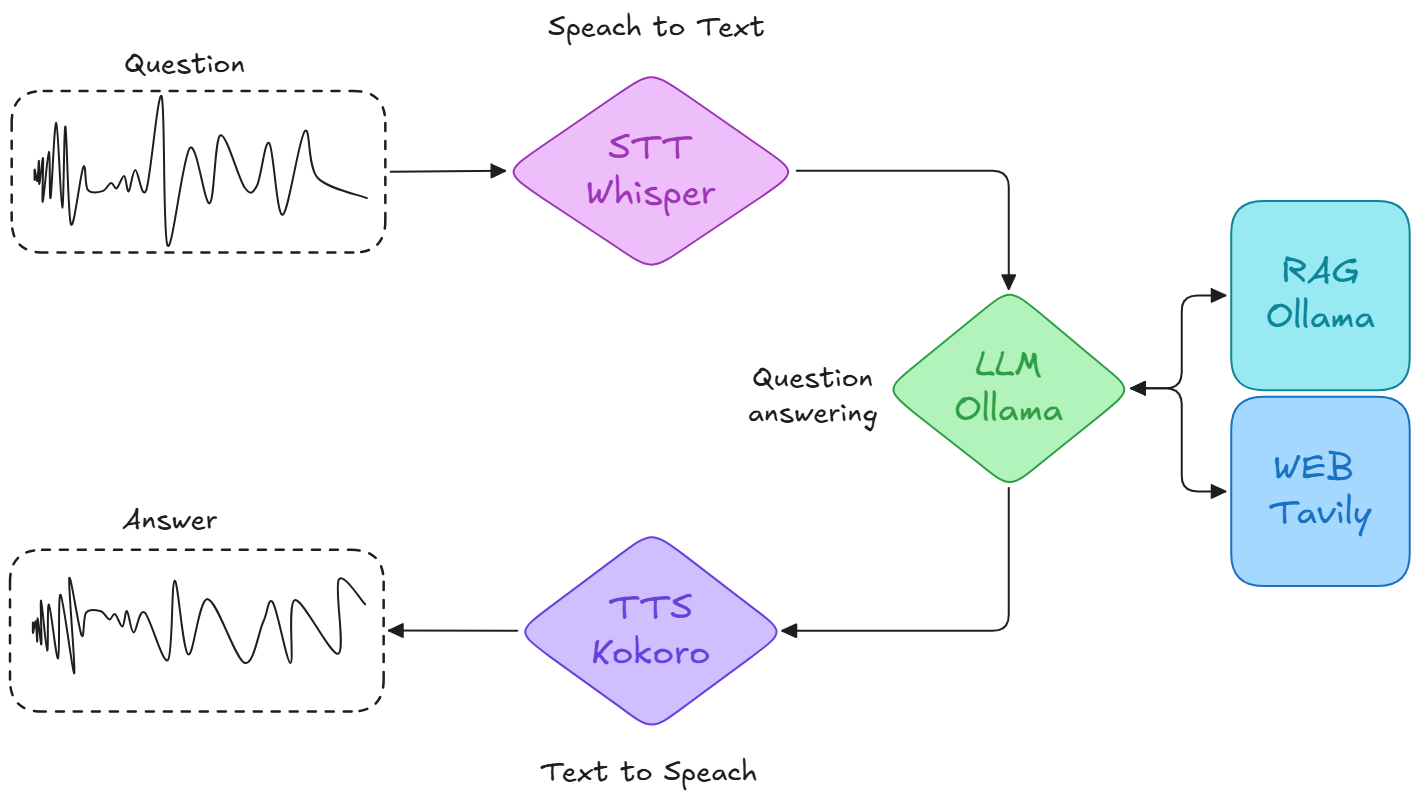
\includegraphics[width=0.5\linewidth]{images/structure_local.png}
    \caption{Estructura del asistente de voz con modelos \textit{locales}.}
    \label{fig:structure_local}
\end{figure}

\subsection{Speech to Text (Whisper)}
Se integró Whisper \cite{radford-whisper-2022} en su variante \texttt{large-v3}, cargado directamente con la librería \texttt{faster-whisper} para aprovechar la cuantización INT8 y reducir la ocupación de VRAM. La llamada al modelo recibe el archivo de audio grabado desde la interfaz y devuelve la transcripción en texto plano, que se pasa directamente al módulo RAG.

El modelo funciona muy bien como se observa en los resultados. La integración es sencilla y eficiente. Durante las pruebas se detecta una limitación práctica: el modelo falla con siglas o nombres propios muy específicos del dominio ('MIARFID' → 'MirFit'; 'PyCatan' → 'PaiKatan'). Estos errores se propagan en cadena, pues si la transcripción es incorrecta el RAG raramente localiza el documento correcto y la respuesta final queda comprometida.

\subsection{RAG (Ollama)}
Todo el componente RAG se orquestó con \textbf{LangChain} \cite{langchain-2025}, aprovechando Ollama \cite{ollama-2023} como backend de inferencia local. Su uso se basa en indexar documentos, recibir la transcripción, recuperar contexto y generar la respuesta. 

\subsubsection{Indexación y persistencia}
Los PDFs (nuestra información / contexto local) se cargan con \texttt{PyPDFLoader} y se trocean con \texttt{RecursiveCharacterTextSplitter} (\texttt{chunk}=1000 chars, \texttt{overlap}=200). Cada chunk se vectoriza con el modelo de embeddings \textbf{mistral-nemo} \cite{mistral-nemo-2024} servido por Ollama y se persiste en \textbf{ChromaDB}. 

Esta parte es de las más importantes, ya que el rendimiento del RAG depende en gran medida de la calidad de la indexación. También por obvias razones de eficiencia, se comprueba si la base de datos ya existe para evitar re-indexaciones innecesarias.

\subsubsection{Evaluación de relevancia}
Antes de que el LLM genere la respuesta final del usuario, se recuperan los $k=10$ chunks más similares a la consulta y se le pasa ese contexto a \textbf{llama3.1} \cite{meta-llama-3-1-2024} con un prompt evaluador para que solo responda 'SÍ' o 'NO':

\begin{lstlisting}[language=Python]
prompt_evaluador = ChatPromptTemplate.from_messages([
    ('system', 'Eres un evaluador de relevancia. Responde estrictamente con una palabra: 'SÍ' o 'NO'.'),
    ('human', f'Pregunta: {pregunta} \n\n Contexto recuperado: {documentos} \n\n ¿Contiene este contexto la información necesaria para responder?')
])
\end{lstlisting}

Esto es únicamente para evaluar si el contexto local es suficiente o no para generar la respuesta. En caso de que el contexto local sea insuficiente o irrelevante, el sistema activa un mecanismo de \textit{fallback} en que utiliza la herramienta \textbf{TavilySearchResults} \cite{tavily-2024} para obtener la información de la web. Para este caso, se ha establecido a 5 el número máximo de resultados que se devolverán por búsqueda y se ha indicado que se realice una búsqueda avanzada.


\subsubsection{Generación de respuesta}
Teniendo el contexto adecuado, en ambos casos, el prompt de la respuesta indica explícitamente al modelo a responder en texto plano sin Markdown, formato imprescindible para que la síntesis de voz no verbalice asteriscos ni guiones:

\begin{lstlisting}[language=Python]
system_prompt = (
    'Eres un asistente de investigación. Responde de forma natural, fluida y concisa, '
    'no des detalles innecesarios y ve directamente al grano. '
    f'La información proviene de {fuente_info}. '
    'IMPORTANTE: No uses negritas, ni asteriscos, ni listas, ni ningún formato markdown. '
    'Escribe todo en un párrafo o párrafos de texto plano, como si fuera una carta o un mensaje de voz.'
    '\n\nContexto: {context}'
)
\end{lstlisting}

\subsection{Text to Speech (Kokoro)}

Una vez el cerebro del sistema genera la respuesta de texto, el último paso es comunicar el feedback al usuario mediante voz. Para ello, se integra Kokoro \cite{hexgrad-kokoro-2025}. Este recibe el texto plano devuelto por el RAG (limpio, sin formato), selecciona la voz deseada y genera el audio directamente en memoria como array \texttt{numpy}, que la interfaz reproduce sin necesidad de escribir archivos intermedios en disco. El proceso completo corre en CPU/GPU de forma transparente según la disponibilidad del sistema.


\section{Implementación Cloud}

La implementación de local a cloud es bastante directa. Se hace uso de la misma lógica implementada en cada componente. Además, gracias a \textbf{LangChain}, al abstraer los proveedores bajo la misma interfaz, basta con cambiar la instancia del modelo para que el RAG completo funcione, reutilizando los mismos prompts, la misma lógica de \textit{fallback} y la misma estructura de orquestación.

La intención inicial es centralizar todos los servicios en \textbf{AWS}, pero problemas de validación de cuenta y suscripciones bloqueadas obligan a diversificar en un collage de proveedores:

\begin{itemize}
    \item \textbf{Groq} \cite{groq-2025}: Nos provee de una versión de Whisper igual a la usada en el entorno local. Además de poder acceder a algunos LLM como \textbf{llama-3.1-8b-instant} para hacer lo mismo que en el entorno local. Las llamadas se realizan mediante el wrapper \texttt{ChatGroq} de LangChain, lo que hizo el cambio completamente transparente a nivel de código.
    \item \textbf{Hugging Face} \cite{huggingface-2025}: los embeddings para indexar todos los documentos se generan con \texttt{sentence-transformers/all-MiniLM-L6-v2} vía la clase \texttt{HuggingFaceEmbeddings}, sustituyendo directamente a los embeddings de Ollama en el paso de indexación y recuperación.
    \item \textbf{AWS Polly} \cite{aws-2025}: se llama al servicio mediante \texttt{boto3}, para que devuelva un audio \texttt{mp3} con el texto proporcionado. Todo parecido a la integración de Kokoro.
\end{itemize}

Esta fragmentación introduce una complejidad operativa notable: cada proveedor gestiona su propia autenticación (API keys, credenciales AWS), cuotas de uso y condiciones de servicio, elevando el esfuerzo de despliegue respecto al entorno local. Toda la experimentación se realiza dentro de los planes gratuitos de cada proveedor, sin llegar al límite de uso en ningún caso. A fecha de Mayo de 2026, existe el riesgo de que alguno de los servicios cambie sus condiciones o limite el acceso, lo cual es inherente a depender de terceros.

\begin{figure}[H]
    \centering
    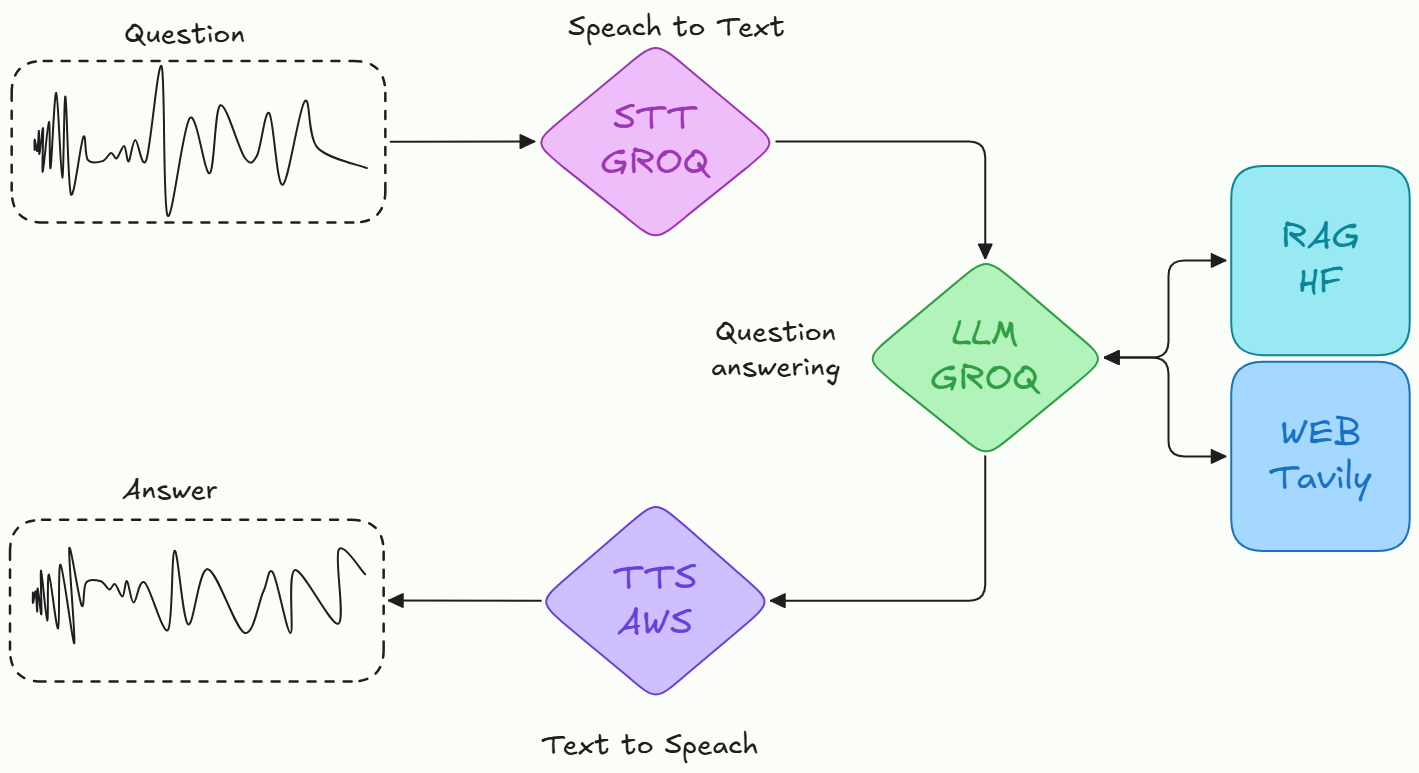
\includegraphics[width=0.5\linewidth]{images/structure_cloud.png}
    \caption{Estructura del asistente de voz con proveedores \textit{cloud}.}
    \label{fig:structure_cloud}
\end{figure}


%%%%%%%%%%%%%%%%%%%%%%%%%%%%%%%%%%%%%%%%%%%%%%%%%%%%%%%%%%%%%%%%%%%%%%%%%%%%%
%                             Resultados y Análisis                                     %
%%%%%%%%%%%%%%%%%%%%%%%%%%%%%%%%%%%%%%%%%%%%%%%%%%%%%%%%%%%%%%%%%%%%%%%%%%%%%

\chapter{Resultados y Análisis}

Una vez implementado todo el sistema en ambos entornos, se diseña un experimento con 30 audios pregrabados, obteniendo 60 ejecuciones (30 por modalidad) para evaluar su rendimiento. 

\section{Metodología de Evaluación}

\begin{itemize}
    \item \textbf{Tiempos:} $T_{total} = T_{STT} + T_{RAG} + T_{TTS}$ (la búsqueda web se excluye por ser igual en ambas).
    \item \textbf{WER:} \textit{Word Error Rate} sobre las transcripciones, normalizadas con \texttt{werpy.normalize} \cite{werpy-2024} (minúsculas, sin puntuación, espacios homogeneizados).
    \item \textbf{RAG Matching Source:} binario (0/1); el sistema usó la fuente correcta (local si el dato estaba en documentos, web si no).
    \item \textbf{RAG Matching Response:} binario (0/1); la respuesta final fue correcta independientemente de la fuente.
    \item \textbf{TTS Score (0–100):} valoración manual de fluidez, pausas lógicas y naturalidad.
\end{itemize}

\section{Resultados}

\begin{table}[H]
\centering
\caption{Métricas obtenidas en la evaluación de los 30 audios.}
\label{tab:results_metrics}
\renewcommand{\arraystretch}{1.2}
\begin{tabular}{@{}lrr@{}}
\toprule
\textbf{Métrica}                  & \textbf{Local} & \textbf{Cloud} \\ \midrule
Transcribe Time (s)               & 3.95           & 0.41           \\
RAG Time (s)                      & 6.04           & 31.98          \\
TTS Time (s)                      & 1.03           & 0.86           \\
\textbf{Total Time (s)}           & \textbf{11.02} & \textbf{33.25} \\ \midrule
Transcription WER (\%)            & 5.22\%         & 6.32\%         \\ \midrule
RAG Matching Source (Raw)         & 24 / 30        & 27 / 30        \\
RAG Matching Response (Raw)       & 19 / 30        & 25 / 30        \\ 
RAG Matching Source (\%)          & 80.00\%        & 90.00\%        \\
RAG Matching Response (\%)        & 63.33\%        & 83.33\%        \\ \midrule
\textbf{TTS Score (0–100)}        & \textbf{50}    & \textbf{90}    \\ \bottomrule
\end{tabular}
\end{table}

\begin{figure}[H]
    \centering
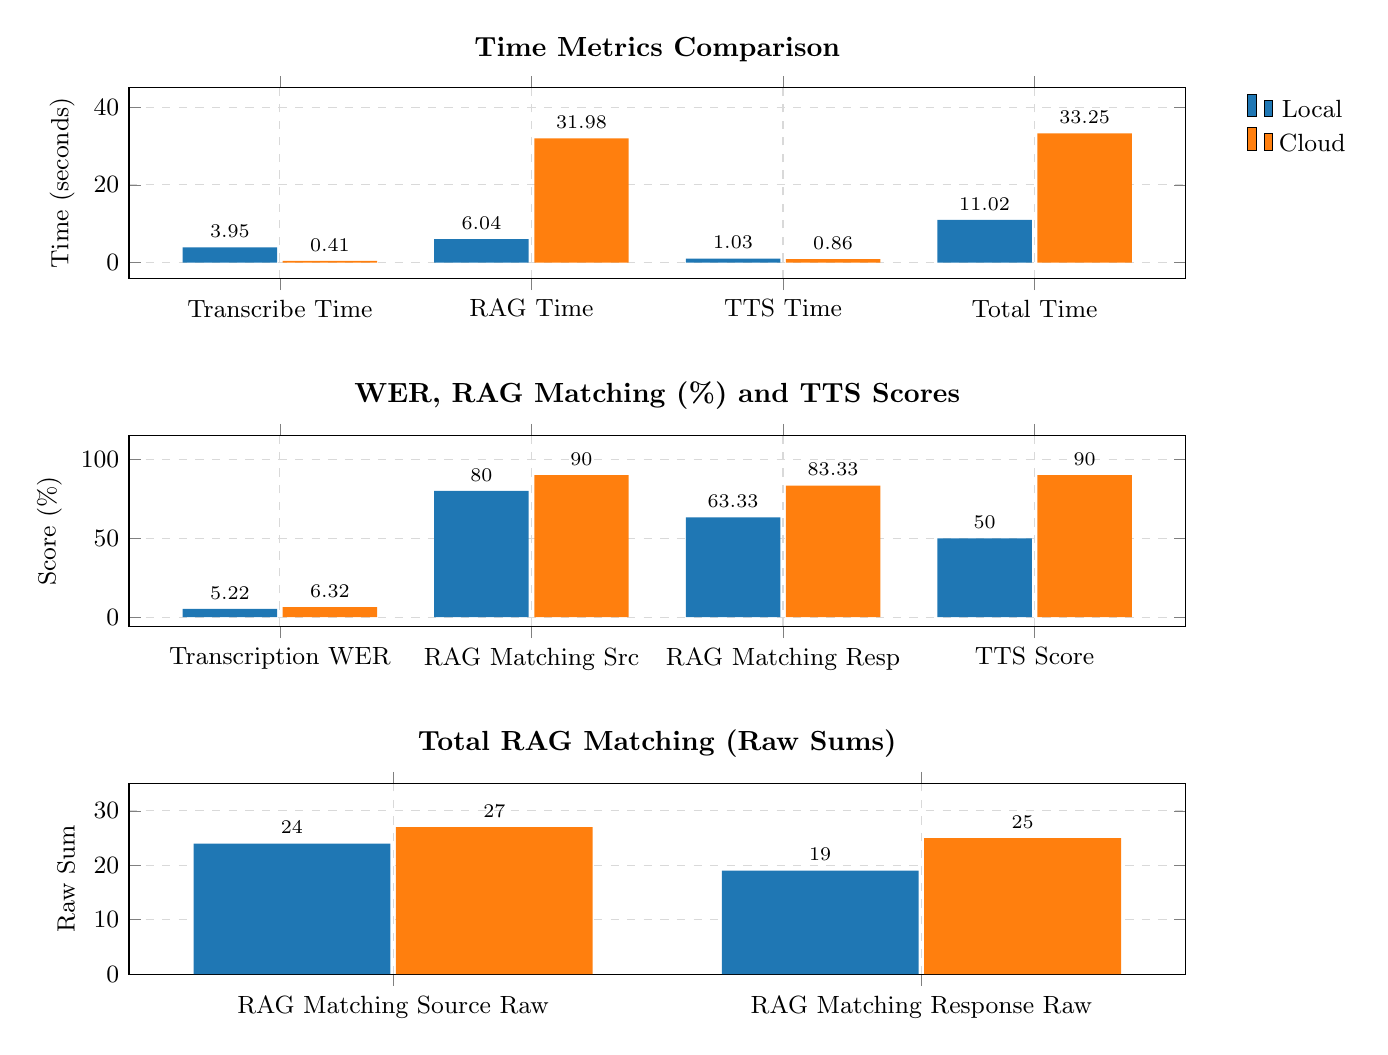
\begin{tikzpicture}
    \begin{groupplot}[
        group style={
            group size=1 by 3,
            vertical sep=2cm,
            x descriptions at=edge bottom,
        },
        ybar,
        width=15cm,
        height=4cm,
        /pgf/bar width=1.2cm,
        enlarge x limits=0.2,
        ylabel style={font=\small},
        tick label style={font=\small},
        nodes near coords,
        every node near coord/.append style={font=\scriptsize, /pgf/number format/fixed, /pgf/number format/precision=2},
        legend style={at={(1.05,1)}, anchor=north west, draw=none, font=\small},
        symbolic x coords={trans_time, rag_time, tts_time, total_time, wer, matching_src, matching_resp, tts_score, src_raw, resp_raw},
        xtick=data,
        grid=major,
        grid style={dashed, gray!30}
    ]
    \nextgroupplot[
        title=\textbf{Time Metrics Comparison},
        ylabel={Time (seconds)},
        xticklabels={Transcribe Time, RAG Time, TTS Time, Total Time},
        xtick={trans_time, rag_time, tts_time, total_time},
        ymax=45
    ]
    \addplot[fill=localblue, draw=none] coordinates {(trans_time,3.95) (rag_time,6.04) (tts_time,1.03) (total_time,11.02)};
    \addplot[fill=cloudorange, draw=none] coordinates {(trans_time,0.41) (rag_time,31.98) (tts_time,0.86) (total_time,33.25)};
    \legend{Local, Cloud}
    \nextgroupplot[
        title=\textbf{WER, RAG Matching (\%) and TTS Scores},
        ylabel={Score (\%)},
        xticklabels={Transcription WER, RAG Matching Src, RAG Matching Resp, TTS Score},
        xtick={wer, matching_src, matching_resp, tts_score},
        ymax=115
    ]
    \addplot[fill=localblue, draw=none] coordinates {(wer,5.22) (matching_src,80.00) (matching_resp,63.33) (tts_score,50)};
    \addplot[fill=cloudorange, draw=none] coordinates {(wer,6.32) (matching_src,90.00) (matching_resp,83.33) (tts_score,90)};
    \nextgroupplot[
        title=\textbf{Total RAG Matching (Raw Sums)},
        ylabel={Raw Sum},
        xticklabels={RAG Matching Source Raw, RAG Matching Response Raw},
        xtick={src_raw, resp_raw},
        ymax=35,
        ymin=0,
        /pgf/bar width=2.5cm,
        enlarge x limits=0.5
    ]
    \addplot[fill=localblue, draw=none] coordinates {(src_raw,24) (resp_raw,19)};
    \addplot[fill=cloudorange, draw=none] coordinates {(src_raw,27) (resp_raw,25)};
    \end{groupplot}
\end{tikzpicture}
    \caption{Contraste de resultados: tiempos, porcentajes de acierto y conteo crudo (de las 30 pruebas de cada uno, cuántas han acertado).}
    \label{fig:results_plots}
\end{figure}

\section{Comparativa por fase: Calidad e implicación}


\begin{itemize}
    \item \textbf{STT:} Ambas opciones son casi \textit{plug and play}. La nube es $\approx10 \times$ más rápida (0.41s vs 3.95s), pero ninguna representa un cuello de botella crítico. WER prácticamente idéntico (5.22\% local vs 6.32\% cloud). Ambos con la limitación común identificada de siglas y nombres específicos.
    
    \item \textbf{RAG:} LangChain abstrae por completo la diferencia entre Ollama y los proveedores cloud, permitiendo reutilizar el mismo código cambiando solo la instancia del modelo. La nube supera en precisión final (83.33\% vs 63.33\%) pero es $\approx \times 5$ más lenta en el tiempo de orquestación (31.98s vs 6.04s). El evaluador local (llama3.1) mostró mayor tendencia a descartar contexto válido y derivar búsquedas a la web innecesariamente, especialmente en preguntas sobre figuras conocidas (Messi). 
    
    Esta diferencia de precisión se debe a los modelos de embeddings: se observa la diferencia de calidad entre mistral-nemo (local) y sentence-transformers (cloud), que impacta directamente en la recuperación de contexto relevante. Estos factores, al igual que otros, se deben optimizar para poder hacer uso de este sistema en caso de querer escalar a un entorno de producción.
    
    \item \textbf{TTS:} AWS supera ampliamente a Kokoro en naturalidad: pausas lógicas, inflexiones y fluidez claramente superiores, con latencia incluso menor (0.86s vs 1.03s). Kokoro es pequeño y eficiente, pero suena plano en comparación.
    
    \item \textbf{Complejidad de integración:} El entorno local es más simple de desplegar (una sola máquina, sin gestión de API keys ni cuotas). La solución cloud multiproveedor introduce complejidad burocrática (autenticación, cuotas, políticas de cada servicio) que eleva el esfuerzo de despliegue pese a su mejor rendimiento en calidad.
    
    \item \textbf{Hardware y privacidad:} 
    Además, hay que tener en cuenta otras consideraciones no cuantificables pero relevantes a la hora de elegir entre una opción u otra: La privacidad de los datos, las dependencias de terceros, la escalabilidad, la flexibilidad para cambiar componentes o la necesidad de hardware específico. 
    
    En este sentido: La opción \textbf{local} ofrece máxima \textbf{privacidad} y control total sobre los datos, \textbf{sin depender de terceros} ni de sus políticas. Sin embargo, \textbf{requiere hardware} potente (VRAM/RAM) y puede ser más difícil de escalar o mantener. La \textbf{nube} externaliza la gestión y el mantenimiento, ofrece \textbf{escalabilidad} instantánea, calidad superior en algunos casos (ya que son modelos privados de empresas) y ofrece un \textbf{gran catálogo de modelos} (aunque a nivel opensource cada vez tenemos más opciones), pero a costa de la privacidad y la dependencia de terceros.

    Sobre todo, destacar la privacidad y la dependencia del entorno local que requiere VRAM y RAM considerables. Sin hardware suficiente, la nube es la única opción viable. A cambio, la nube externaliza los datos a terceros y depende de planes y políticas que pueden cambiar. 
    
\end{itemize}

\subsection{Curiosidades y fallos observados}
\begin{itemize}
    \item \textbf{STT:} Siglas de dominio específico transcritas incorrectamente por los ASRs, ('MIARFID'→'MirFit', 'PyCatan'→'PaiKatan') provocan fallos en cadena en el RAG que no permiten recuperar el contexto correcto y comprometen la respuesta final.
    \item \textbf{RAG — fuente incorrecta:} El evaluador ignoraba contexto local válido y forzaba búsqueda web (frecuente en preguntas sobre Messi). La cosa es que de normal, cuando el LLM se queda con contexto insuficiente, alucina la respuesta. En cambio, al salir a la web, aunque no sea lo ideal, es más probable que acierte. Esto se refleja en la diferencia de precisión entre ambos entornos.
    \item \textbf{RAG — inconsistencia web:} Preguntas con respuesta subjetiva o no determinista ('¿raza de perro más peluda?') generaban respuestas distintas en cada ejecución ('Chow Chows', 'Akitas', 'Pullis'...) dependiendo de la fuente consultada por Tavily. Véase Figura~\ref{fig:web_search_inconsis}.
\end{itemize}

\begin{figure}[H]
    \centering
    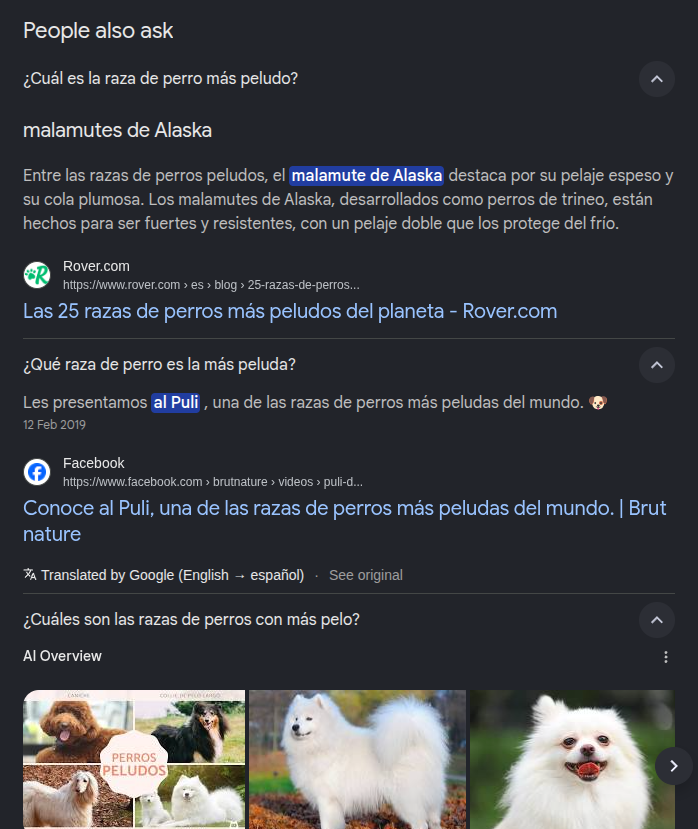
\includegraphics[width=0.4\linewidth]{images/web-seach-inconsistency.png}
    \caption{Inconsistencia del evaluador RAG: prefiere la web ignorando datos locales disponibles.}
    \label{fig:web_search_inconsis}
\end{figure}

\section{Tiempos de respuesta}
Como se aprecia en los tiempos de la figura \ref{fig:results_plots}, el entorno en la nube tiene una latencia de respuesta global muy alta (principalmente por el excesivo tiempo consumido en la orquestación RAG). Pese a que en tareas aisladas como la transcripción de audio (STT) la nube demuestra ser notablemente más rápida frente a la ejecución local, el tiempo final se resiente. 

Ya que el feedback del sistema es uno de los factores más críticos para la experiencia del usuario, tardar tanto es un gran inconveniente, de media, el sistema cloud es hasta 3 veces más lento que en el entorno local. 

Las diferentes partes terminan dando un resultado similar y al final se consiguen respuestas correctas en ambos casos, pero la espera es un factor que puede llegar a ser molesto para el usuario (más incluso que la calidad de voz por ejemplo).


\section{Estructura sugerida}
Para finalizar, se propone una estructura de sistema híbrida que combine lo mejor de ambos mundos (entre lo que se ha probado): \textbf{usar proveedores cloud para el reconocimiento de voz (STT) y la síntesis de voz (TTS) y llevar gestión del RAG de forma local. }

De esta forma, se consigue la latencia más baja (según las pruebas $7.31s$, como referencia, Alexa responde en 1 a 4 segundos), se mantiene la máxima privacidad con respecto a los datos procesados, y se obtiene una calidad de voz sobresaliente. Además, el sistema RAG local puede ser tan potente como la máquina lo permita, y no se ve limitado por las restricciones de los proveedores externos.

El único inconveniente de esta arquitectura sería la limitación en la elección de LLMs. Pero con la creciente variedad de modelos, cada vez más pequeños y eficientes, esto no debería ser un gran problema para tareas 'tan simples' como responder preguntas concretas basadas en un contexto específico.

%%%%%%%%%%%%%%%%%%%%%%%%%%%%%%%%%%%%%%%%%%%%%%%%%%%%%%%%%%%%%%%%%%%%%%%%%%%%%%
%                   CONCLUSIONES Y TRABAJOS FUTUROS
%%%%%%%%%%%%%%%%%%%%%%%%%%%%%%%%%%%%%%%%%%%%%%%%%%%%%%%%%%%%%%%%%%%%%%%%%%%%%%

\chapter{Conclusiones y trabajos futuros}

Queda demostrado que es totalmente viable desplegar un flujo completo de interacción por voz tanto en local como en la nube, con resultados sólidos en tiempos competentes. Las conclusiones clave por bloque son:

\begin{itemize}
    \item \textbf{STT:} La nube es más rápida (0.41s vs 3.95s) pero con WER prácticamente idéntico (5.22\% local vs 6.32\% cloud). Ambos con limitaciones similares en siglas y nombres específicos.
    \item \textbf{RAG:} La nube ofrece mayor tasa de acierto en respuesta final por el modelo de embeddings (83.33\% vs 63.33\%), pero con latencia disparada y pérdida de privacidad. El evaluador local alucina cuando su contexto es escaso, pero abusar del \textit{fallback} web expone al sistema a información inestable o no determinista. Algo fácilmente arreglable con un modelo de embeddings local más potente, sin tener que recurrir a la nube.
    \item \textbf{TTS:} AWS es ganador indiscutible en naturalidad (score 90 vs 50) con latencia igual o menor que Kokoro. A no ser que la privacidad sea prioritaria, la nube gana en esta fase.
    \item \textbf{Despliegue:} Lo local garantiza privacidad total y simplicidad; la nube aporta un catálogo más potente pero con complejidad burocrática, dependencia de terceros e incertidumbre sobre sus futuras políticas. Ahora sí, los planes gratuitos actuales son suficientes para uso personal. Por lo que sin pagar (ni suscripciones ni hardware), la nube ofrece un sistema completo.
\end{itemize}

La elección depende de las prioridades: sin hardware potente, la nube es la única opción; con máquina capaz y prioridad en privacidad, el entorno local es preferible; buscando un compromiso, la arquitectura híbrida (STT+TTS cloud, RAG local) es la más adecuada.

\section{Trabajos futuros}

\begin{itemize}
    \item \textbf{Optimización y Streaming:} El sistema más rápido actual ronda los 7s de respuesta. Usar modelos más ligeros y generar texto/audio en tiempo real (\textit{streaming}) reduciría drásticamente la latencia percibida.
    \item \textbf{Wake Word:} Sistema 'siempre escuchando' (estilo 'OK Google') que mantenga el micrófono en bajo consumo y active el flujo pesado solo al detectar la palabra clave.
    \item \textbf{Hardware empotrado:} Portar el sistema a Raspberry Pi o NVIDIA Jetson para un altavoz autónomo, asumiendo que las limitaciones de este hardware obligarán a delegar ciertos servicios a la nube.
    \item \textbf{Ampliación del agente:} Incorporar más herramientas MCP y volúmenes de datos mayores para superar el modo pregunta-respuesta, lo que podría requerir de LLMs más grandes.
\end{itemize}

%%%%%%%%%%%%%%%%%%%%%%%%%%%%%%%%%%%%%%%%%%%%%%%%%%%%%%%%%%%%%%%%%%%%%%%%%%%%%%%
%                                                                             %
%                                BIBLIOGRAFIA                                 %
%                                                                             %
%%%%%%%%%%%%%%%%%%%%%%%%%%%%%%%%%%%%%%%%%%%%%%%%%%%%%%%%%%%%%%%%%%%%%%%%%%%%%%%
\cleardoublepage
\printbibliography

%%%%%%%%%%%%%%%%%%%%%%%%%%%%%%%%%%%%%%%%%%%%%%%%%%%%%%%%%%%%%%%%%%%%%%%%%%%%%%%
%                                                                             %
%                                 APÉNDICESS                                  %
%                                                                             %
%%%%%%%%%%%%%%%%%%%%%%%%%%%%%%%%%%%%%%%%%%%%%%%%%%%%%%%%%%%%%%%%%%%%%%%%%%%%%%%

\APPENDIX


%%%%%%%%%%%%%%%%%%%%%%%%%%%%%%%%%%%%%%%%%%%%%%%%%%%%%%%%%%%%%%%%%%%%%%%%%%%%%%
%                       EJEMPLOS DE CADA TIPO DE FACTURA                     %
%%%%%%%%%%%%%%%%%%%%%%%%%%%%%%%%%%%%%%%%%%%%%%%%%%%%%%%%%%%%%%%%%%%%%%%%%%%%%%

% \chapter{Apéndice correspondencia notebooks}
% \label{appendix:notebooks}
% ...

%%%%%%%%%%%%%%%%%%%%%%%%%%%%%%%%%%%%%%%%%%%%%%%%%%%%%%%%%%%%%%%%%%%%%%%%%%%%%%%
%                              FIN DEL DOCUMENTO                              %
%%%%%%%%%%%%%%%%%%%%%%%%%%%%%%%%%%%%%%%%%%%%%%%%%%%%%%%%%%%%%%%%%%%%%%%%%%%%%%%
\end{document}

